% Template for ICME-2010 paper; to be used with:
%          spconf.sty  - ICASSP/ICIP LaTeX style file, and
%          IEEEbib.bst - IEEE bibliography style file.
% --------------------------------------------------------------------------
\documentclass{article}
\usepackage{graphicx}
\usepackage{spconf_ICME,amsmath,epsfig,fancyhdr}
\setlength{\paperwidth}{215.9mm} \setlength{\hoffset}{-9.7mm}
\setlength{\oddsidemargin}{0mm} \setlength{\textwidth}{184.3mm}
\setlength{\columnsep}{6.3mm} \setlength{\marginparsep}{0mm}
\setlength{\marginparwidth}{0mm} \setlength{\paperheight}{279.4mm}
\setlength{\voffset}{-7.4mm} \setlength{\topmargin}{0mm}
\setlength{\headheight}{0mm} \setlength{\headsep}{0mm}
\setlength{\topskip}{0mm} \setlength{\textheight}{235.2mm}
\setlength{\footskip}{12.4mm} \setlength{\parindent}{1pc}


\ICMEfinalcopy % *** Uncomment this line for the final submission

\def\ICMEPaperID{****} % *** Enter the ICME Paper ID here
\def\httilde{\mbox{\tt\raisebox{-.5ex}{\symbol{126}}}}

% Pages are numbered in submission mode, and unnumbered in camera-ready
\ifICMEfinal\pagestyle{empty}\fi


\begin{document}\sloppy

% Example definitions.
% --------------------
\def\x{{\mathbf x}}
\def\L{{\cal L}}


% Title.
% ------
\title{AN APPLICATION FOR FINDING AND CLASSIFYING FRUIT IN IMAGES}
%
% Single address.
% ---------------
\name{Eric Henderson and Nick Kamper}
\address{Rose-Hulman Institute of Technology}


\maketitle
% insert page header and footer here for IEEE PDF Compliant
\thispagestyle{fancy} \fancyhead{} \lhead{}
%\lfoot{978-1-4244-7493-6/10/\$26.00~\copyright2010 IEEE} \cfoot{}
%\rfoot{ICME 2010}
\renewcommand{\headrulewidth}{0pt}
\renewcommand{\footrulewidth}{0pt}




%
\begin{abstract}
In this paper, we describe a technique for finding and classifying fruit in a given set of images using a manually-tuned thresholding based on HSV color space and filtering the noise to acceptable levels. With the technique we describe, we were able to correctly identify all of the fruit in one of our images, with only minor errors in the other three given images. 
\end{abstract}
%
\begin{keywords}
image classification,thresholding,median filtering
\end{keywords}
%
\section{Introduction}
\label{sec:intro}

The subject of this paper is an application that will find and classify fruit in a given set of images using color thresholding in HSV space. After thresholding, our technique will filter the noise using morphological operators, median filters, and average connected region area. 

The fruits appearing the given data are \textbf{apples}, \textbf{bananas}, and \textbf{oranges}. Our thresholds were manually tuned for these given images, but our technique and code could be adapted to handle other images. 


\section{Process}
\label{sec:process}
\subsection{Overview}
\label{subsec:process:overview}

The first step in finding the fruit is to convert the image to the HSV image space.  Then, simple thresholding is used to remove the background from the image.  Next, thresholding is used again, but this time to find individual types of fruit.  These initial fruit masks are enhanced by using morphological operators, such as erosion and dilation, as well as a median filter.  After obtaining a mask of each fruit, connected objects can be used to find separate pieces of fruit.  To filter out any noise that may have gotten past the filtering, the area of each connected region is computed in order to determine any outliers.  These outliers are then removed.  Finally, the centroid of each piece of fruit and the number of pieces of each type are calculated.

\subsection{Thresholding}
Our technique involves using two different levels of thresholding: a threshold to remove the background of the image and then a set of thresholds to find the different fruits. This technique allows the foreground filters (for finding the fruits) to be less selective, as those filters will not have to deal with false-positives in the background.

\subsection{Enhancing the mask}
After thresholding, there is a rough mask of the area where the fruit is. However, these masks contain a significant amount of noise. Our technique uses two methods to reduce the impact of this noise prior to finding regions: a median filter and morphological operations. 

First, a median filter, using a 5x5 square, is applied. The median filter is suitable for ``salt and pepper" noise, which we determined was one of the more common types of noise seen in thresholded images. Next, a morphological close operation, consisting of an erosion and dilation, is applied to the image using a 3x3 diamond, equivalent to a four-neighborhood. After these operations, the mask is relatively free of major noise and holes.

\subsection{Finding connected regions}
After the mask is enhanced, our technique will find the connected regions within the image using MATLAB's \texttt{bwlabel} using a four-neighborhood. \texttt{bwlabel} returns a matrix consisting of 0, 1, ..., n in each cell, corresponding to the regions. These regions are then split up into individual masks and normalized into binary masks. 

\subsection{Removing more noise}
At this point, each mask contains a single connected region. However, there are still some regions that correspond to noise in the mask. To reduce this noise further, our technique will then calculate the average area of each mask and removes those masks which has an area significantly smaller or larger than the average region size. This concludes the processing of the masks by our technique. 

\section{Training data}
\subsection{Thresholding values}
\label{subsec:process:filters}
\subsubsection{Background capturing thresholds}
\label{subsubsec:process:filters:background}
~\\
\textbf{Filter 1}
\[0.000 <= H <= 1.000\]
\[0.275 <= S <= 0.425\]
\[0.100 <= V <= 0.450\]\\
~
\textbf{Filter 2}
\[0.150 <= H <= 0.450\]
\[0.000 <= S <= 0.900\]
\[0.000 <= V <= 0.225\]\\
~
\textbf{Filter 3}
\[0.100 <= H <= 0.275\]
\[0.125 <= S <= 0.350\]
\[0.000 <= V <= 1.000\]\\

\subsubsection{Fruit capturing thresholds}
\label{subsubsec:process:filters:fruit}
~\\
\textbf{Apple}
\[0.925 <= H\ \textbf{OR}\ H <= 0.100\]
\[0.600 <= S <= 1.000\]
\[0.050 <= V <= 0.500\]\\
~
\textbf{Banana}
\[0.120 <= H <= 0.250\]
\[0.500 <= S <= 1.000\]
\[0.450 <= V <= 1.000\]\\
~
\textbf{Orange}
\[0.060 <= H <= 0.110\]
\[0.600 <= S <= 1.000\]
\[0.500 <= V <= 0.950\]\\

\subsection{Filters and Morphological Operators}
\label{subsec:process:filtmorph}
\begin{enumerate}
\item Median filter using a 5x5 square
\item Close operator using a 3x3 diamond (equivalent to four-neighborhood)
\end{enumerate}

\section{Results}
\subsection{mixed\_fruit1.tiff}
For the first image, \texttt{mixed\_fruit1.tiff}, we were able to successfully identify the correct number of fruits.
\subsubsection{Data}
Apple (7 found)\\~\\
\begin{tabular}{ | r | r | r | }
\hline
\textbf{X} & \textbf{Y} & \textbf{Size}\\
\hline
143.3259 & 91.8101 & 316\\
\hline
48.3462 & 129.7372 & 312\\
\hline
208.7509 & 196.4874 & 277\\
\hline
186.0201 & 246.1253 & 447\\
\hline
218.3883 & 330.7949 & 273\\
\hline
60.6172 & 446.1513 & 337\\
\hline
65.4917 & 477.8017 & 242\\
\hline
\end{tabular}
~\\~\\~\\
Banana (6 found)\\~\\
\begin{tabular}{ | r | r | r | }
\hline
\textbf{X} & \textbf{Y} & \textbf{Size}\\
\hline
218.5945 & 159.2760 & 587\\
\hline
52.0207 & 230.0284 & 387\\
\hline
55.4043 & 272.9688 & 512\\
\hline
242.5063 & 387.5781 & 474\\
\hline
279.2613 & 497.4947 & 750\\
\hline
187.6559 & 602.1696 & 401\\
\hline
\end{tabular}
~\\~\\~\\
Orange (7 found)\\~\\
\begin{tabular}{ | r | r | r | }
\hline
\textbf{X} & \textbf{Y} & \textbf{Size}\\
\hline
143.6724 & 64.2783 & 406\\
\hline
187.7799 & 272.5670 & 418\\
\hline
231.4619 & 280.6571 & 420\\
\hline
53.6546 & 376.9342 & 304\\
\hline
200.0660 & 409.3198 & 394\\
\hline
202.3764 & 445.0029 & 348\\
\hline
179.7903 & 566.8041 & 434\\
\hline
\end{tabular}

\subsubsection{Images}
Original image\\~\\
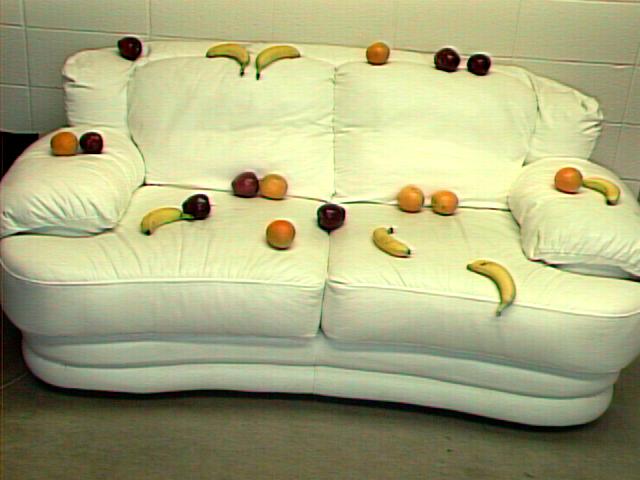
\includegraphics[width=2in]{mixed_fruit1.png}\\~\\
Original mask\\~\\
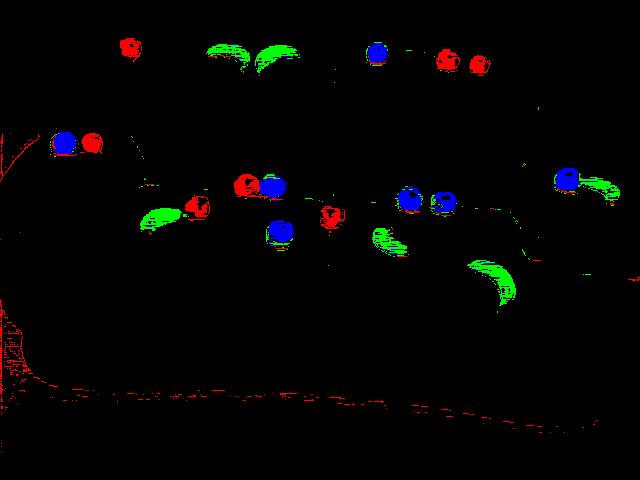
\includegraphics[width=2in]{mixed_fruit1_step1.png}\\~\\
Clean mask\\~\\
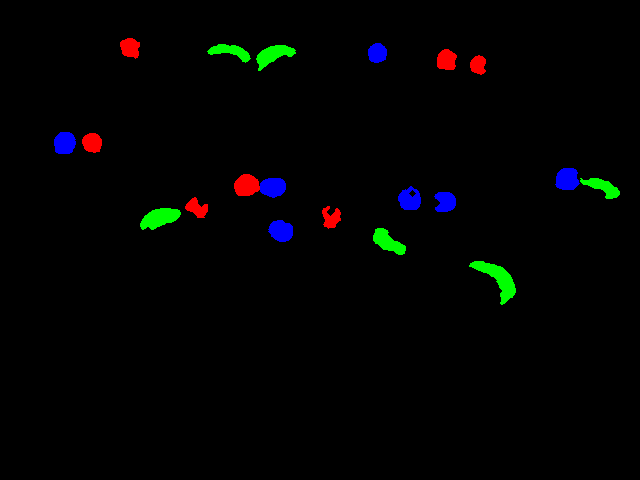
\includegraphics[width=2in]{mixed_fruit1_step2.png}\\~\\

\subsection{mixed\_fruit2.tiff}
For the second image, \texttt{mixed\_fruit2.tiff}, we were able to successfully identify the correct number of bananas and oranges, but detected an extra apple. 
\subsubsection{Data}
Apple (7 found)\\~\\
\begin{tabular}{ | r | r | r | }
\hline
\textbf{X} & \textbf{Y} & \textbf{Size}\\
\hline
369.5518 & 160.4705 & 1932\\
\hline
319.0113 & 266.0188 & 1864\\
\hline
437.8009 & 270.6967 & 211\\
\hline
44.5030 & 284.1810 & 1000\\
\hline
407.1295 & 324.2635 & 1985\\
\hline
94.5485 & 484.9597 & 1537\\
\hline
284.8667 & 596.4200 & 300\\
\hline
\end{tabular}
~\\~\\~\\
Banana (6 found)\\~\\
\begin{tabular}{ | r | r | r | }
\hline
\textbf{X} & \textbf{Y} & \textbf{Size}\\
\hline
388.4214 & 68.4231 & 2361\\
\hline
176.4266 & 64.5710 & 2494\\
\hline
289.7583 & 195.3878 & 2437\\
\hline
290.3219 & 343.8662 & 2653\\
\hline
175.9601 & 467.8580 & 2557\\
\hline
319.9872 & 563.1305 & 2352\\
\hline
\end{tabular}
~\\~\\~\\
Orange (6 found)\\~\\
\begin{tabular}{ | r | r | r | }
\hline
\textbf{X} & \textbf{Y} & \textbf{Size}\\
\hline
92.3523 & 58.6880 & 1388\\
\hline
33.0721 & 234.4446 & 1498\\
\hline
412.9493 & 268.4607 & 2229\\
\hline
414.2446 & 391.5243 & 2081\\
\hline
419.1797 & 511.5228 & 2215\\
\hline
266.6702 & 586.3969 & 1716\\
\hline
\end{tabular}

\subsubsection{Images}
Original image\\~\\
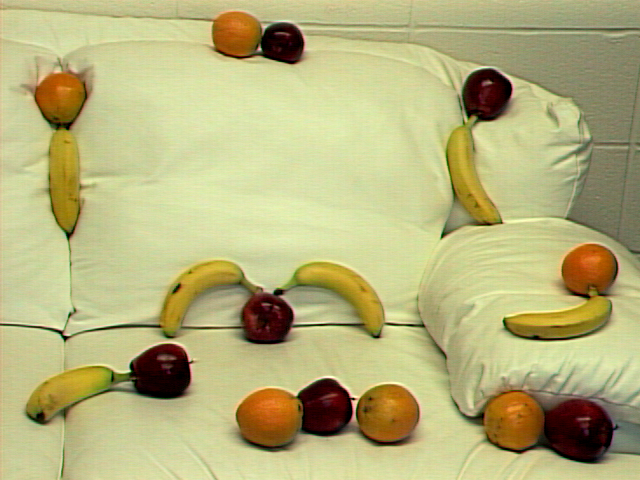
\includegraphics[width=2in]{mixed_fruit2.png}\\~\\
Original mask\\~\\
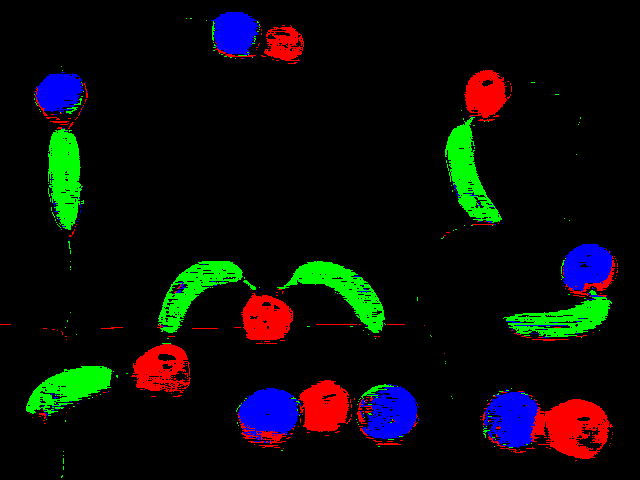
\includegraphics[width=2in]{mixed_fruit2_step1.png}\\~\\
Clean mask\\~\\
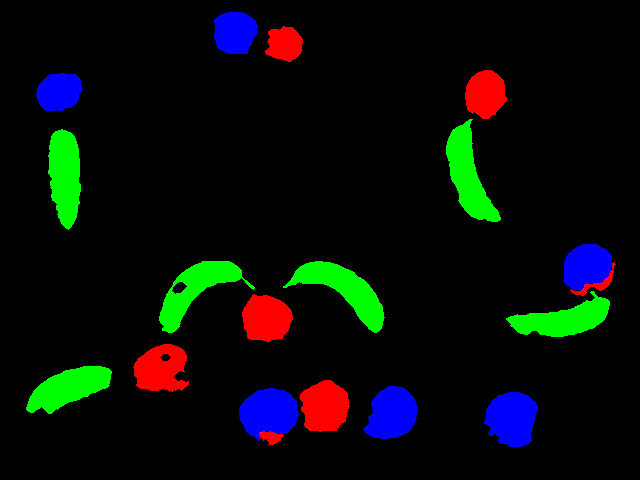
\includegraphics[width=2in]{mixed_fruit2_step2.png}\\~\\

\subsection{mixed\_fruit3.tiff}
For the third image, \texttt{mixed\_fruit3.tiff}, we were able to successfully identify the correct number of apples, but there was an extra banana and an extra orange.
\subsubsection{Data}
Apple (8 found)\\~\\
\begin{tabular}{ | r | r | r | }
\hline
\textbf{X} & \textbf{Y} & \textbf{Size}\\
\hline
299.3567 & 36.1389 & 5657\\
\hline
201.2441 & 59.2207 & 639\\
\hline
418.7965 & 148.1597 & 5542\\
\hline
287.5883 & 161.4418 & 3619\\
\hline
175.9445 & 184.4902 & 3874\\
\hline
176.0630 & 461.1911 & 2365\\
\hline
298.6333 & 466.7226 & 3079\\
\hline
383.6635 & 539.9577 & 4583\\
\hline
\end{tabular}
~\\~\\~\\
Banana (7 found)\\~\\
\begin{tabular}{ | r | r | r | }
\hline
\textbf{X} & \textbf{Y} & \textbf{Size}\\
\hline
227.2263 & 99.3108 & 5476\\
\hline
242.3035 & 262.0122 & 4913\\
\hline
76.8940 & 241.2440 & 5501\\
\hline
297.6278 & 293.5087 & 1150\\
\hline
160.2507 & 389.4048 & 5034\\
\hline
61.9554 & 491.2378 & 4579\\
\hline
232.1099 & 575.9033 & 5004\\
\hline
\end{tabular}
~\\~\\~\\
Orange (8 found)\\~\\
\begin{tabular}{ | r | r | r | }
\hline
\textbf{X} & \textbf{Y} & \textbf{Size}\\
\hline
165.8371 & 47.7669 & 3886\\
\hline
199.9871 & 133.1239 & 1162\\
\hline
357.5691 & 190.3717 & 4651\\
\hline
179.8290 & 280.9192 & 3912\\
\hline
333.2355 & 277.6628 & 1210\\
\hline
304.6516 & 325.1719 & 1309\\
\hline
242.8631 & 424.1327 & 4018\\
\hline
362.9017 & 456.0160 & 5067\\
\hline
\end{tabular}

\subsubsection{Images}
Original image\\~\\
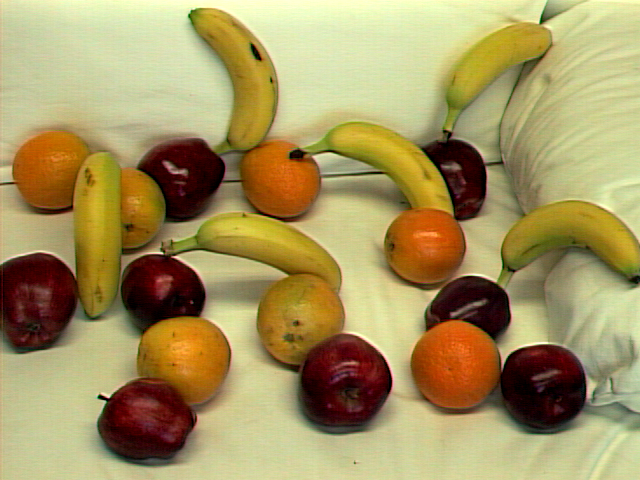
\includegraphics[width=2in]{mixed_fruit3.png}\\~\\
Original mask\\~\\
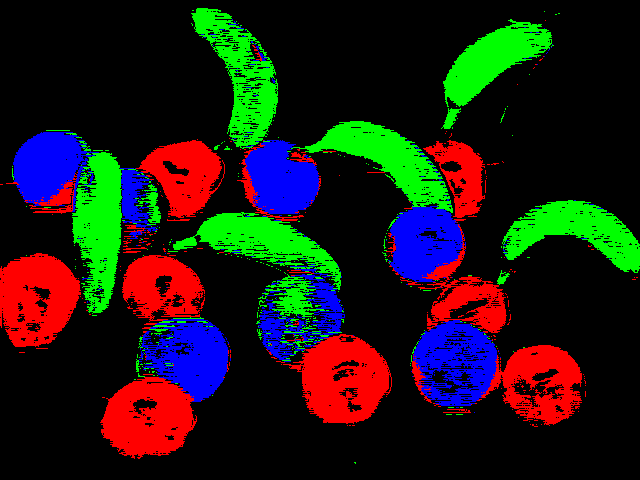
\includegraphics[width=2in]{mixed_fruit3_step1.png}\\~\\
Clean mask\\~\\
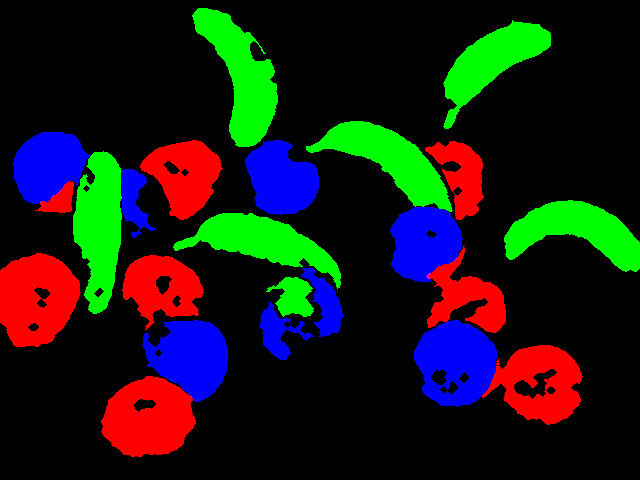
\includegraphics[width=2in]{mixed_fruit3_step2.png}\\~\\

\subsection{fruit\_tray.tiff}
For the fourth image, \texttt{fruit\_tray.tiff}, we were unable to identify the correct number of fruit as a result of our thresholding giving data that is too noisy for our filtering code to retain as fruits. This could be a result of the thresholds being used were not tuned for this application or that the filtering was too aggressive. 
\subsubsection{Data}
Apple (8 found)\\~\\
\begin{tabular}{ | r | r | r | }
\hline
\textbf{X} & \textbf{Y} & \textbf{Size}\\
\hline
310.8944 & 111.0427 & 1477\\
\hline
164.9810 & 138.8308 & 1897\\
\hline
264.5828 & 162.8235 & 2368\\
\hline
373.3612 & 196.3010 & 299\\
\hline
124.6049 & 220.7136 & 405\\
\hline
203.7126 & 221.0749 & 414\\
\hline
265.7575 & 288.9318 & 763\\
\hline
228.2927 & 438.5954 & 2108\\
\hline
\end{tabular}
~\\~\\~\\
Banana (1 found)\\~\\
\begin{tabular}{ | r | r | r | }
\hline
\textbf{X} & \textbf{Y} & \textbf{Size}\\
\hline
82.9100 & 212.5757 & 667\\
\hline
\end{tabular}
~\\~\\~\\
Orange (1 found)\\~\\
\begin{tabular}{ | r | r | r | }
\hline
\textbf{X} & \textbf{Y} & \textbf{Size}\\
\hline
229.4551 & 126.0366 & 12867\\
\hline
\end{tabular}

\subsubsection{Images}
Original image\\~\\
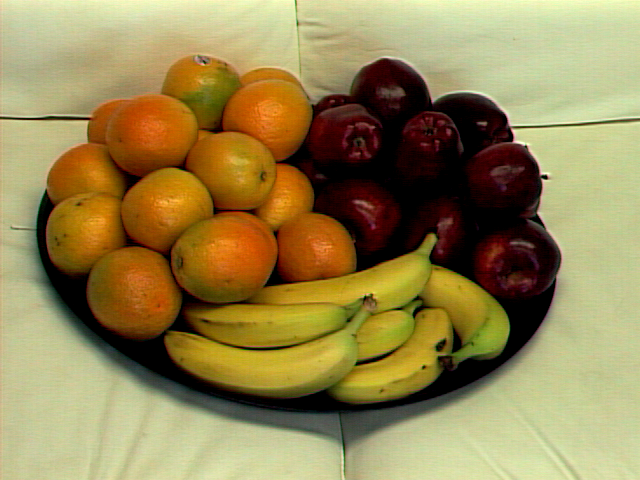
\includegraphics[width=2in]{fruit_tray.png}\\~\\
Original mask\\~\\
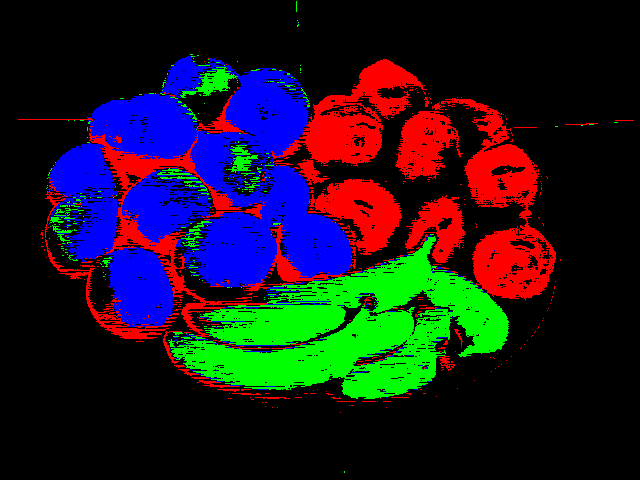
\includegraphics[width=2in]{fruit_tray_step1.png}\\~\\
Clean mask\\~\\
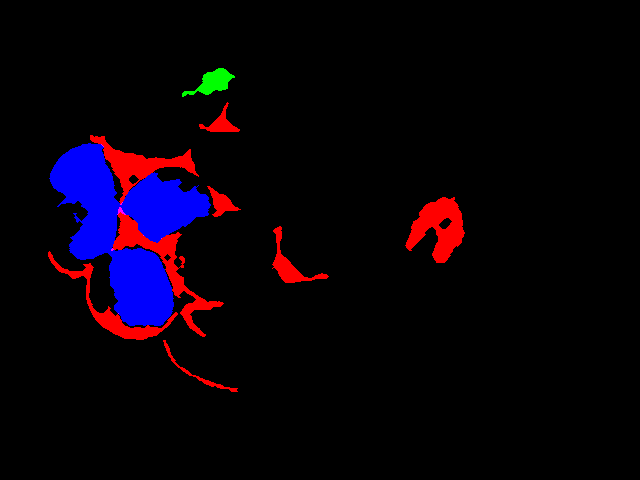
\includegraphics[width=2in]{fruit_tray_step2.png}\\~\\

\section{Future Work}
There are various techniques that we could use to improve our technique in the future.
\subsection{Canny-inspired Adaptive Two-Level Thresholding}
One potential idea would be to use multi-level thresholding as a way of capturing more area of the fruits while limiting the amount of additional erroneous data being introduced. The primary idea is to use a ``high" threshold to pick out regions that have a high probability of being a fruit, then a ``low" threshold would be applied to the neighbors of those ``high" threshold pixels and then to other neighboring ``low" pixels. This would allow those high probability areas to ``grow" out and encapsulate the entire fruit.
\subsection{Contrast Improvement}
Another potential idea would be to increase the contrast of the image after applying the thresholds to remove the background. This would allow our technique to have a larger difference between neighboring colors, such as the case with the red in the apples, the orange in the oranges, and the yellow in the bananas, which are neighboring colors in the hue band of HSV.    
\subsection{Shape/Edge Detection}
Another potential idea would be to use edge detection to pick out regions that could potentialy be a fruit and use shape detection to determine the type of fruit. This could have better results when combined with color. 

\end{document}
